\chapter{Theoretical Foundations of Geometrical Computer Vision}\label{chap:theoretic_found}

% In your case, it could for instance contain the math of camera models, the theory of feature point detection and matching, motion field models, in your case in particular the model of a moving plane, parameterization of motion in terms of rotation matrices and translation vectors, and how they are computed from a set of feature point correspondences 

\section{Coordinate Frames}
We are working with camera images, which are 2-D representations of points in a 3-D world. We also have different points of reference: in the real world, according to the camera etc. It is thus of utmost importance to define the coordinate frames we will be using to avoid confusion.\bigskip

First of all, there is the image itself, the \newterm{image coordinate frame ICF}. This is a 2-D frame with x-axis and y-axis along the horizontal axis and vertical axis of the image respectively. The unit of these coordinates is measured in pixels and the center of the frame is at the top left of the image. The image frame is shown in \autoref{fig:im_frame}\bigskip

\begin{figure}
    \centering
    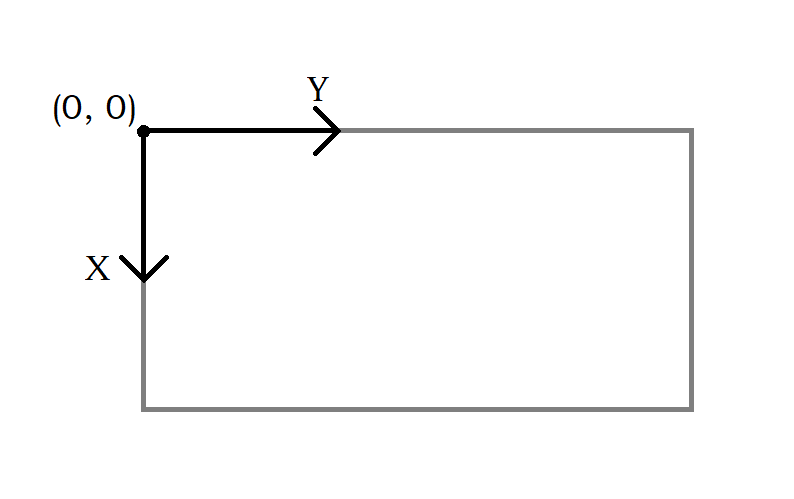
\includegraphics[width=1\textwidth]{figures/image_frame.png}
    \caption{Image frame}
    \label{fig:im_frame}
\end{figure}

Secondly, there is the \newterm{vehicle coordinate frame VCF}. This is a right-handed 3-D coordinate system. The center of the frame is located at the bottom center of the car. The x-axis is pointing right, the y-axis is pointing down and the z-axis is leaving the car perpendicular to the car in the direction of the front of the car. \bigskip

Closely related, we have the \newterm{camera coordinate frame CCF}. This is a similar 3-D coordinate system, but as I stated before, the camera is mounted slightly tilted at the side of the car. With respect to the camera, the x-axis is once again pointing right, the y-axis pointing down and the z-axis leaving the camera perpendicular to the camera in the direction of the view. These two coordinate frames are shown in \autoref{fig:cam_frame}, with the cube being an abstract way of showing the car.\bigskip

\begin{figure}
    \centering
    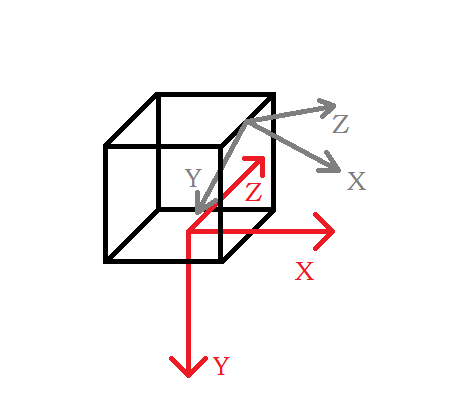
\includegraphics[width=1\textwidth]{figures/camera_frame.png}
    \caption{Vehicle and camera coordinate frame}
    \label{fig:cam_frame}
\end{figure}

The fourth and last coordinate frame is the \newterm{world coordinate frame WCF}. This is also a right-handed 3-D coordinate system and to keep things simple, the center is located at center of the VCF at frame 1. The difference is that the frame is rotated around the z-axis so the y-axis is pointing upwards and the x-axis is pointing left. See \autoref{fig:world_frame} where the cube is once again the car in its initial position.\bigskip

\begin{figure}
    \centering
    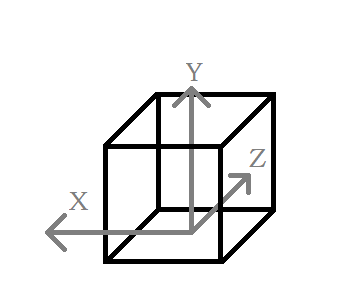
\includegraphics[width=1\textwidth]{figures/world_frame.png}
    \caption{World coordinate frame}
    \label{fig:world_frame}
\end{figure}

As we are working with three different coordinate frames, it's important to know how to transfer points from one frame to another. We'll discuss this at length in a later section.

\subsection{Relation of different coordinate frames}
Working with different coordinate frames can be tricky, to avoid any confusion I will define the transformation equations between the different coordinate frames. 

\subsubsection{VCF to CCF}
The first thing we have to do is define how the center of the VCF is translated to the center of the CCF, therefore we define $\vt_{VC}$ as the translation from the VCF to the CCF. Looking at \autoref{fig:cam_frame} from the point of view of the VCF, the center is translated along the x-axis to the right thus being positive, along the y-axis to the left thus being negative. This is of course all depending on where the camera is mounted exactly, but from \autoref{fig:footage_example} it is clear that in our case the camera is mounted on the upper right side of the car. Whether the camera is moved along the z-axis and in which direction is unknown. This gives the following definition:
\begin{equation}
    \vt_{VC} = \begin{pmatrix}
         t_{VC,1} \\ -t_{VC,2} \\ t_{VC,3}
     \end{pmatrix} 
\end{equation}

Secondly, we need to have a look at the rotation, how a rotation matrix works is explained in \autoref{ssec:rotmat}. The rotation from VCF to CCF is defined like this (for a detailed explanation on how rotation matrices work, see \autoref{ssec:rotmat}):

\begin{equation}
    \MR_{VC} = \MR_z(\phi_{VC})\cdot\MR_y(\psi_{VC})\cdot\MR_x(\theta_{VC})
\end{equation}

Thus, to transform a point $P_V = (P_{V1}, P_{V2}, P_{V3})^T$ in the VCF to it's corresponding coordinates $P_C = (P_{C1}, P_{C2}, P_{C3})^T$ in the CCF, the following transformation is done:
\begin{equation}
    \begin{pmatrix}
        P_{C1} \\ P_{C2}\\ P_{C3}
    \end{pmatrix} = \MR_{VC}\begin{pmatrix}
        P_{V1} \\ P_{V2}\\ P_{V3}
    \end{pmatrix} + \vt_{VC} 
\end{equation}

To go from the CCF to the VCF, it is only logical to do the reverse transformation: first subtracting $\vt_{VC}$ followed by a rotation inverse to $\MR_{VC}$.

\subsubsection{VCF to WCF}
When switching between the VCF and the WCF there are different scenario's. Unlike in the previous section, the VCF and WCF have no fixed transformation. The VCF will move relative to the WCF (which is what we will be trying to track).\bigskip

Before the car has moved, the VCF and WCF will be located at the same point by definition of the WCF. Thus the translation vector $\vt_{VW}$ equals $(0, 0, 0)^T$. The WCF equals the VCF at frame 0 rotated around the z-axis over 180 degrees or $\pi$. This gives us the following rotation matrix:
\begin{equation}
    \MR_{VW} = \MR_z(\pi)\cdot\MR_y(0)\cdot\MR_x(0)
\end{equation}
or
\begin{equation}
    \MR_{VW} = \begin{pmatrix}
        -1 & 0 & 0 \\
        0 & -1 & 0 \\
        0 & 0 & 1
    \end{pmatrix}
\end{equation}

Resulting in the following conversion from $P_V = (P_{V1}, P_{V2}, P_{V3})^T$ to $P_W = (P_{W1}, P_{W2}, P_{W3})^T$:

\begin{equation}\label{eq:VW}
    \begin{pmatrix}
        P_{W1} \\ P_{W2}\\ P_{W3}
    \end{pmatrix} = \MR_{VW}\begin{pmatrix}
        P_{V1} \\ P_{V2}\\ P_{V3}
    \end{pmatrix}
\end{equation}

When the vehicle has already moved from its original starting point, this transformation must be accounted for. To go from the VCF to the WCF, first do the inverse transformation from $VCF_n$ to $VCF_0$ and then rotate following \autoref{VW}.

\subsubsection{CCF to WCF}
To go from the CCF to the WCF, it suffices to concatenate the two previous discussed transformation: going from the CCF to the VCF and then going to the WCF.

\section{Motion Parameters}
Every 3-D rigid motion can be decomposed into two components, each of which have three degrees of freedom. The displacement in this plane is called the translation and can be expressed by the translation vector $\vt$. The second parameter is the rotation, this can be expressed with the rotation matrix $\MR$. Additionally, when a motion is happening on a flat surface we can define this plane uniquely, the normal vector $\vn$ does this.\bigskip

\subsection{Rotation Matrix}\label{ssec:rotmat}
A 3-D rotation can always be described by a sequence of 3 partial rotations, a yaw, a pitch and a roll. It is important to note that the decomposition from rotation matrix to its components is done according to a convention. This convention states the order in which the rotations are done, if these are switched, the decomposition will be wrong. The convention I will use is the Tait-Bryan convention as follows: pitch, yaw, roll, \autoref{eq:rotation} shows this.\bigskip
\begin{figure}
    \centering
    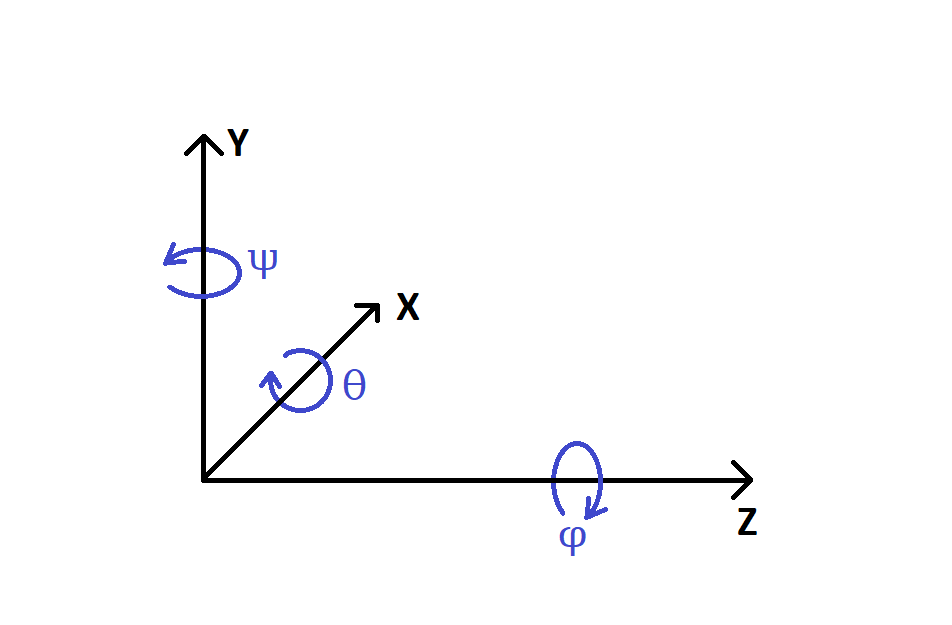
\includegraphics[width=1\textwidth]{figures/yaw_pitch_roll.png}
    \caption{Yaw, pitch and roll}
    \label{fig:rotations}
\end{figure}

\autoref{fig:rotations} shows these rotation components. $\psi$, $\theta$ and $\phi$ are yaw, pitch and roll respectively. As it is a right handed system, we have the following conventions:
\begin{itemize}
    \item When $\psi$ is positive, there is a rotation to the left.
    \item When $\theta$ is positive, there is an upward rotation.
    \item When $\phi$ is positive, there is a clockwise rotation.
\end{itemize}
This is all when looking forward from the center alongside the Z-axis.\bigskip

Each of these rotation components can be defined by a $3\times3$ matrix:
\begin{equation}
    \MR_y(\psi) = \begin{pmatrix}
        \cos\psi & 0 & \sin\psi \\
        0 & 1 & 0 \\
        -\sin\psi & 0 & \cos\psi
    \end{pmatrix}
\end{equation}
\begin{equation}
    \MR_x(\theta) = \begin{pmatrix}
        1 & 0 & 0 \\
        0 & \cos\theta & -\sin\theta \\
        0 & \sin\theta & \cos\theta \\
    \end{pmatrix}
\end{equation}
\begin{equation}
    \MR_z(\phi) = \begin{pmatrix}
        \cos\phi & -\sin\phi & 0 \\
        \sin\phi & \cos\phi & 0 \\
        0 & 0 & 1
    \end{pmatrix}
\end{equation}
To get the rotation matrix $\MR$, we multiply the yawn, pitch and roll like this:
\begin{equation} \label{eq:rotation}
    \MR = \MR_z(\phi)\cdot\MR_y(\psi)\cdot\MR_x(\theta)
\end{equation}
\begin{equation*}
    = \begin{pmatrix}
    \cos\psi\cos\phi & \sin\theta\sin\psi\cos\phi - \cos\theta\sin\phi & \cos\theta\sin\psi\cos\phi + \sin\theta\sin\phi \\
    \cos\psi\sin\phi & \sin\theta\sin\psi\sin\phi + \cos\theta\cos\phi & \cos\theta\sin\psi\sin\phi - \sin\theta\cos\phi \\
    -\sin\psi          & \sin\theta\cos\psi                                  & \cos\theta\cos\psi \\
  \end{pmatrix} 
\end{equation*}

\subsection{Translation Vector}
A translation vector is a $3\times1$ vector of the form $\vt = (t_1, t_2, t_3)^T$. The vector describes the translation along the three different axes. When point $P = (P_1, P_2, P_3)^T$ undergoes a translation described by $\vt$ you get the following:
\begin{equation}
    P' = P + \vt = \begin{pmatrix}
        P_1 + t_1 \\ P_2 + t_2 \\ P_3 + t_3
    \end{pmatrix}
\end{equation}

\section{Motion Description}
\subsection{Motion equation}
We have talked about motion and the motion parameters. Each frame-to-frame motion will be described using these parameters in a motion equation.\bigskip

To define this equation, take a point with the following coordinates in the CCF: $X = (X_1, X_2, X_3)^T$. After the camera moved, this same point $X$ has now the following coordinates in the CCF $X' = (X'_1, X'_2, x'_3)^T$. The transformation from any $X$ to its corresponding $X'$ can be described by the same equation:
\begin{equation}\label{eq:motion}
    \begin{pmatrix}
        X_1\\ X_2\\ X_3
    \end{pmatrix} =  \MR \begin{pmatrix}
        X'_1\\ X'_2\\ X'_3
    \end{pmatrix}+ \vt
\end{equation}

\subsubsection{Homogeneous coordinates}
In what follows, we'll use homogeneous coordinates instead of Cartesian coordinates. The use of Homogeneous coordinates makes some formulas easier to work with and lets us represent projective transformations by a matrix. \bigskip

To write the motion equation from \autoref{eq:motion} in Homogeneous coordinates, we take $P_1 = (X_1, Y_1, Z_1, 1)^T$ and $P_2 = (X_2, Y_2, Z_2, 1)^T$ and come to the following equation:
\begin{equation}
    \begin{pmatrix}
        X_2 \\ Y_2 \\ Z_2 \\ 1
    \end{pmatrix} = \begin{pmatrix}
        \MR & 0 \\
        0 & 0
    \end{pmatrix} \begin{pmatrix}
        X_1 \\ Y_1 \\ Z_1 \\ 1
    \end{pmatrix} + \begin{pmatrix}
        t_1 \\ t_2 \\ t_3 \\ 1
    \end{pmatrix}
\end{equation}
which can be rewritten as
\begin{equation}
    \begin{pmatrix}
        X_2 \\ Y_2 \\ Z_2 \\ 1
    \end{pmatrix} = \begin{pmatrix}
        \MR & \vt \\
        0 & 1
    \end{pmatrix} \begin{pmatrix}
        X_1 \\ Y_1 \\ Z_1 \\ 1
    \end{pmatrix}
\end{equation}
This matrix characterises the transformation or motion that occurred between two frames. Based on these transformation matrices, the position of the camera (and thus the car) can be determined by concatenating the transformations.

\section{Camera model}\label{sec:cammodel}\footnote{Knowledge of this section was primarily gained by the lecture slides of R. Mester \cite{computer_vision}.}
As we work with 2-D images that are a representation of a 3-D world, there are some things to be said about the projection from 3-D to 2-D. The camera used and its properties are important factors in determining motion.

\subsection{Pinhole camera model}
\autoref{fig:cammodel} shows the pinhole camera model. $C$ is the perspective center of the camera, the plane $E$ is the plane on which the 3-D world is projected upon. $H$ is called the principal point, it is the perpendicular projection of $C$ onto $E$, this axis is called the optical axis. $f$ is a constant based on the properties of the camera.\bigskip

Take point $P$ in the 3-D world, its coordinates can be described with respect to camera coordinate frame with $C$ as its center. When a picture is taken, the $P$ is projected on $E$ resulting in point $p$. $P$ with coordinates $X$, $Y$ and $Z$ is transformed to $p$ with coordinates $x$, $y$ and $z$. $z$ always equals $f$ as axis $Y_3$ is perpendicular to $E$.\bigskip

\begin{figure}
    \centering
    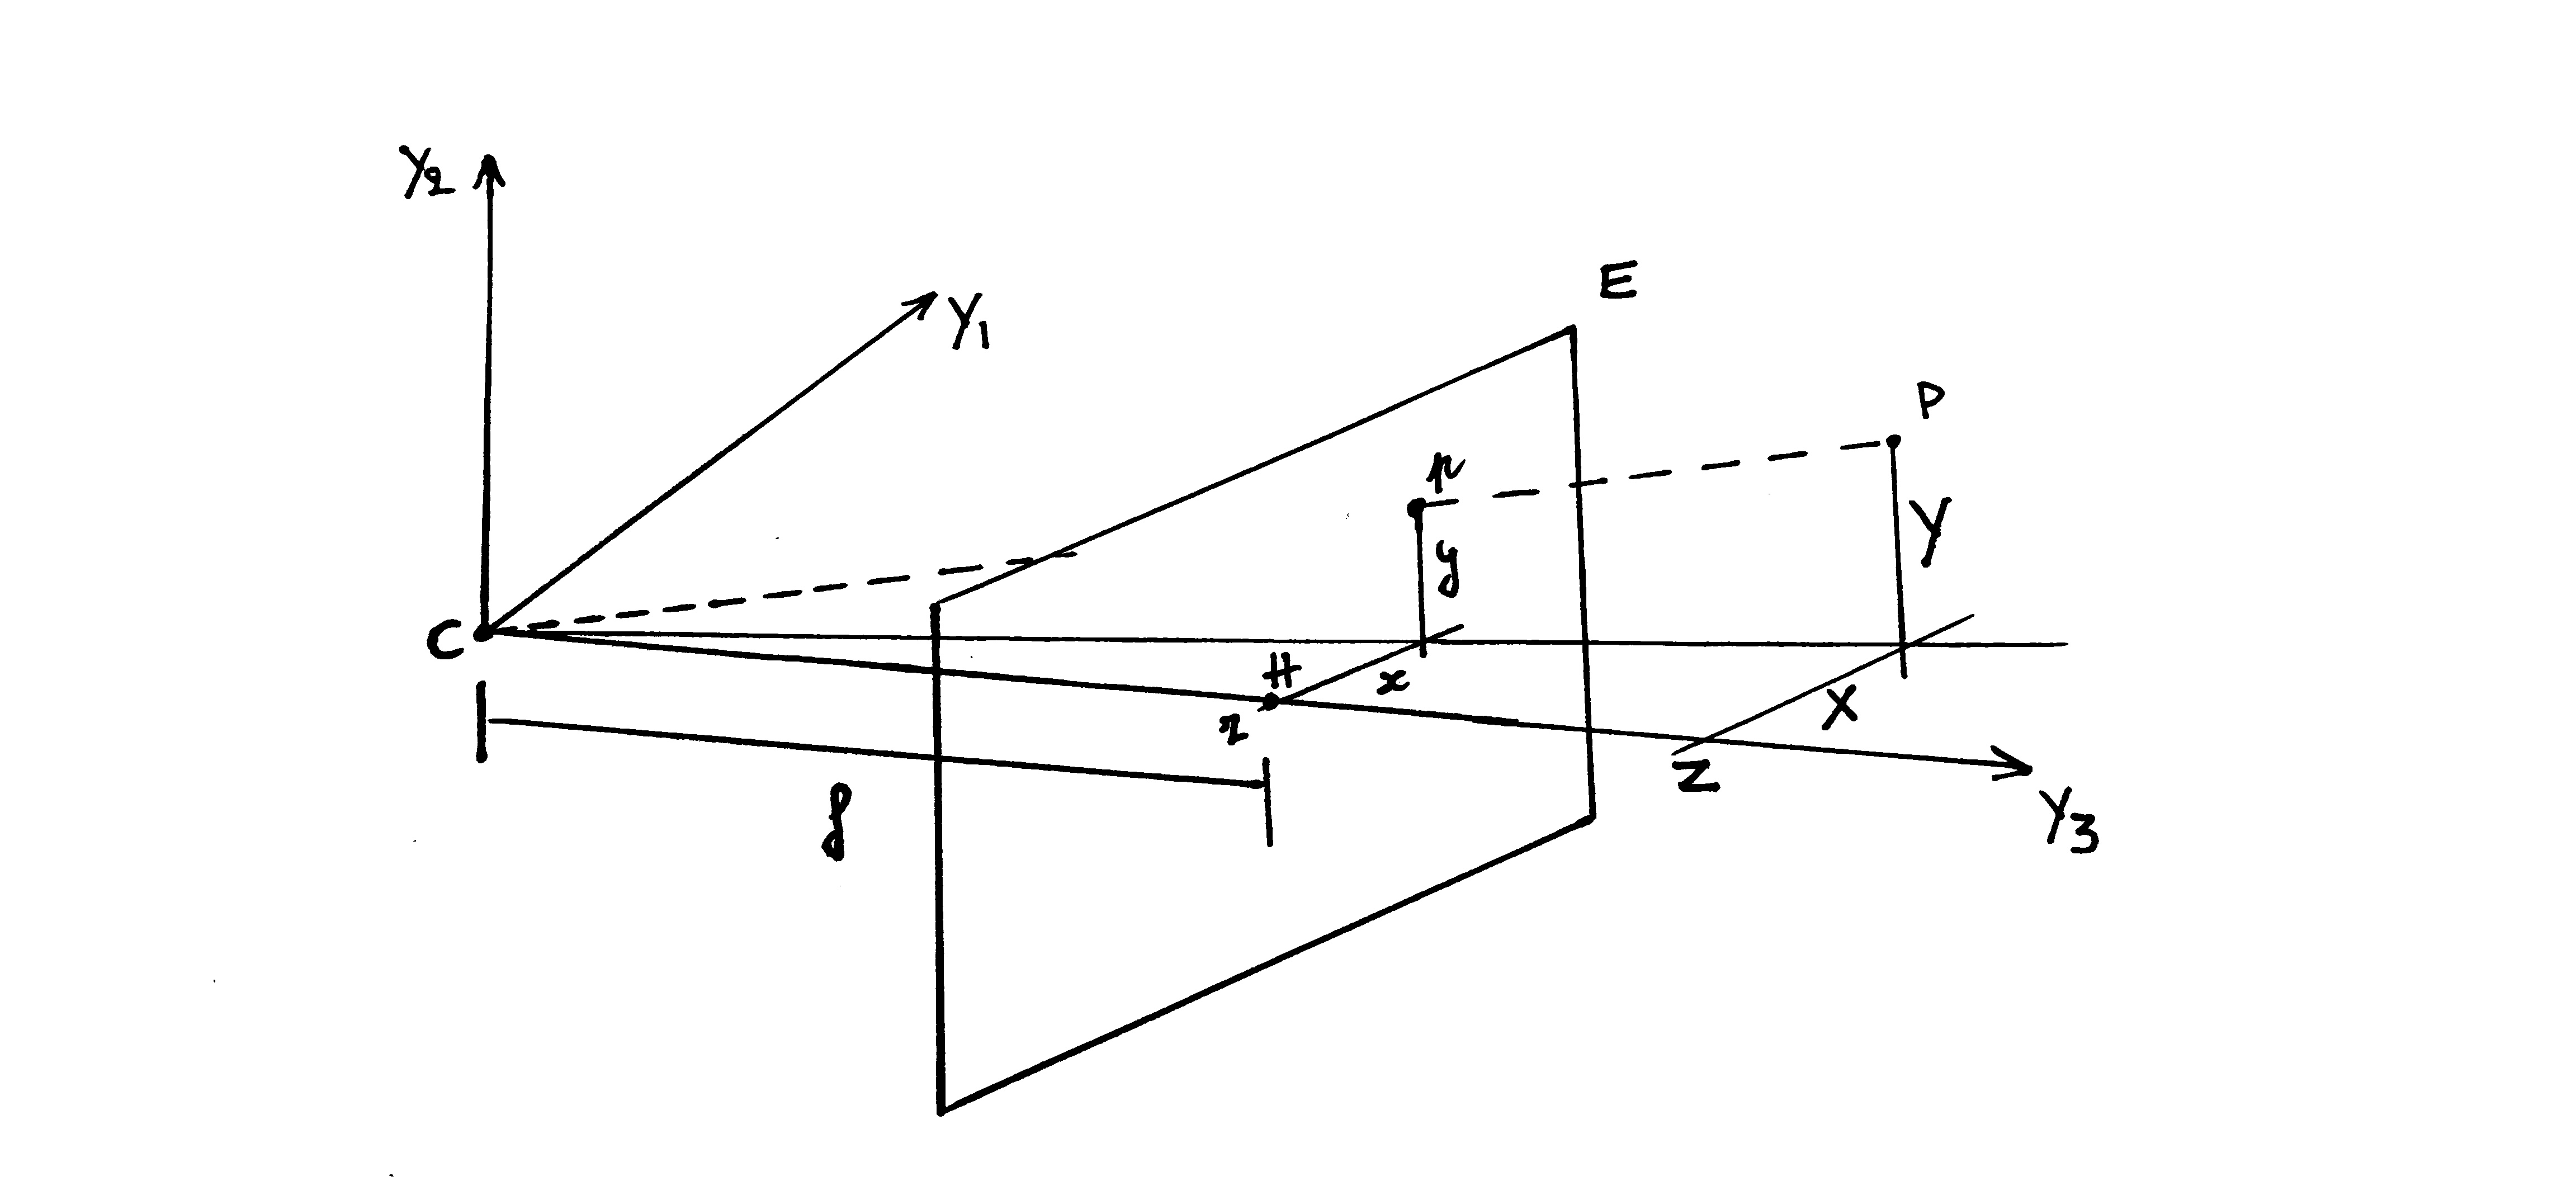
\includegraphics[width=1\textwidth]{figures/camera_model.jpg}
    \caption{Pinhole camera model}
    \label{fig:cammodel}
\end{figure}

We need a way to describe the relationship between $P$ and $p$, the transformation from real world coordinates to camera coordinates. (It is important to note that the next equations are only valid when all the pairs of entities are measured in the same length entities). Given point $P$ with coordinates $(X, Y, Z)^T$ and point $p$ with coordinate $(x, y, z)$ the following relation can be found using the law of similar triangles: 
\begin{equation}
    \frac{x}{X} = \frac{z}{Z} = \frac{f}{Z}
\end{equation}
\begin{equation}
    \frac{y}{Y} = \frac{z}{Z} = \frac{f}{Z}
\end{equation}
Rewriting the equations above, we get the following coordinates for point $\vp$:
\begin{equation}\label{eq:im_proj1}
    x = f\frac{X}{Z}
\end{equation}
\begin{equation}\label{eq:im_proj2}
    y = f\frac{Y}{Z}
\end{equation}
However, these are not linear equations of projection. To keep working with linear equations as long as possible for simplicity, we us an extended vector: 
\begin{equation}\label{eq:exvec}
    \begin{pmatrix}
        x \\ y
    \end{pmatrix} \rightarrow 
    \begin{pmatrix}
        X \\ Y \\ Z/f
    \end{pmatrix}
\end{equation}
To get the original vector $(x, y)^T$ from $(X, Y, Z/f)^T$ we introduce the projection operator 'Proj':
\begin{equation}
    Proj\begin{pmatrix}
        a \\ b \\ c
    \end{pmatrix} :=
    \begin{pmatrix}
        a/c \\ b/c
    \end{pmatrix}
\end{equation}
So the projection from real word coordinates to camera coordinates can be written as follows:
\begin{equation}\label{eq:projection}
    \begin{pmatrix}
        x \\ y
    \end{pmatrix} = Proj
    \begin{pmatrix}
        X \\ Y \\ Z/f
    \end{pmatrix} = 
    \begin{pmatrix}
        f\frac{X}{Z} \\[0.25cm] f\frac{Y}{Z}
    \end{pmatrix}
\end{equation}
This projection operator has an important property: Vectors upon which the projection operator Proj(.) is to be applied may be multiplied by arbitrary factors $\alpha\neq 0$ without changing the result of the projection operation. Proof can be found in the lecture slides of R. Mester \cite{computer_vision}.\bigskip

The vector on the right hand side of \autoref{eq:exvec} can be rewritten as follows:
\begin{equation}
    \begin{pmatrix}
        X \\ Y \\ Z/f
    \end{pmatrix} = 
    \begin{pmatrix}
        1 & 0 & 0\\ 
        0 & 1 & 0\\ 
        0 & 0 & 1/f
    \end{pmatrix}
    \begin{pmatrix}
        X \\ Y \\ Z
    \end{pmatrix}
\end{equation}
Using the property previously discussed of the projection operator which we will use on the vector $(X, Y, Z/f)^T$ we can multiply the vector with factor $f$:
\begin{equation}
    f\begin{pmatrix}
        X \\ Y \\ Z/f
    \end{pmatrix} = f
    \begin{pmatrix}
        1 & 0 & 0\\ 
        0 & 1 & 0\\ 
        0 & 0 & 1/f
    \end{pmatrix}
    \begin{pmatrix}
        X \\ Y \\ Z
    \end{pmatrix}
\end{equation}
\begin{equation}
    = \begin{pmatrix}
        f & 0 & 0\\ 
        0 & f & 0\\ 
        0 & 0 & 1
    \end{pmatrix}
    \begin{pmatrix}
        X \\ Y \\ Z
    \end{pmatrix}   
\end{equation} 
So \autoref{eq:projection} can be written as
\begin{equation}\label{eq:projfull}
    \begin{pmatrix}
        x \\ y
    \end{pmatrix} = Proj\left[
    \begin{pmatrix}
        f & 0 & 0\\ 
        0 & f & 0\\ 
        0 & 0 & 1
    \end{pmatrix}
    \begin{pmatrix}
        X \\ Y \\ Z
    \end{pmatrix} \right]
\end{equation}
To avoid the use of the projection operator, we could rewrite \autoref{eq:projfull} can be rewritten like this:
\begin{equation}
    k
    \begin{pmatrix}
        x \\ y \\ 1
    \end{pmatrix} = 
    \begin{pmatrix}
        f & 0 & 0\\ 
        0 & f & 0\\ 
        0 & 0 & 1
    \end{pmatrix}
    \begin{pmatrix}
        X \\ Y \\ Z
    \end{pmatrix}
\end{equation}
By expressing the point $P$ as a homogeneous vector $(X, Y, Z, 1)^T$ we get the following:
\begin{equation}\label{eq:homproj}
    k
    \begin{pmatrix}
        x \\ y \\ 1
    \end{pmatrix} = 
    \begin{pmatrix}
        f & 0 & 0 & 0\\ 
        0 & f & 0 & 0\\ 
        0 & 0 & 1 & 0
    \end{pmatrix}
    \begin{pmatrix}
        X \\ Y \\ Z \\ 1
    \end{pmatrix}
\end{equation}
\autoref{eq:homproj} shows how to go from the homogeneous real world coordinates, where the origin is the perspective center of the camera $C$, to the camera coordinates, where the origin is the principal point $H$.\bigskip

When working with pictures however, points are pixels on a grid with the origin in the top left corner of the image. So the the points in camera coordinates need to be transformed to image coordinates. Since these coordinate systems are in the same plane and have the same directions, this transformation is a simple translation (assuming both coordinates are given in pixels), whether or not with a minus sign. This means that \autoref{eq:homproj} can be rewritten, adding the translation like this:

\begin{equation}\label{eq:improj}
    k
    \begin{pmatrix}
        x \\ y \\ 1
    \end{pmatrix} = 
    \begin{pmatrix}
        f & 0 & h_x & 0\\ 
        0 & f & h_y & 0\\ 
        0 & 0 & 1 & 0
    \end{pmatrix}
    \begin{pmatrix}
        X \\ Y \\ Z \\ 1
    \end{pmatrix}
\end{equation}
As stated before, when working with these equations, all entities should be measured in the same length entities. For now, this is not the case, $f$ is a value commonly measured in millimeters and image coordinates are measured in pixels. This means that \autoref{eq:improj} is not valid using the values we currently have for $f$ and $H$.\bigskip

To solve this problem, we should transform one of the units to the other unit's length entity. As we are primarily working with images, converting everything to pixels is the best way.\bigskip

To do this, we look at the side view of the camera model, as seen in \autoref{fig:fov}. The Field of View $F$ is a value directly related to $f$ and can be found in the data sheet from the camera that is used (the subscript H and V denote the horizontal and vertical Field of View respectively). To calculate the height of the image, we can use basic trigonometry. In a right-angled triangle the tangent of a corner is equal to the length of the opposite side divided by the length of the adjacent side, in our case this means:
\begin{equation}
    \tan(F_V/2) = \frac{h/2}{f}
\end{equation}\label{eq:fovv}
solving for $h$:
\begin{equation}
    h = 2f*\tan(F_V/2)
\end{equation}
Analogous, we can find the width $w$ of the image like this:
\begin{equation}\label{eq:fovh}
    w = 2f*\tan(F_H/2)
\end{equation}
\begin{figure}
    \centering
    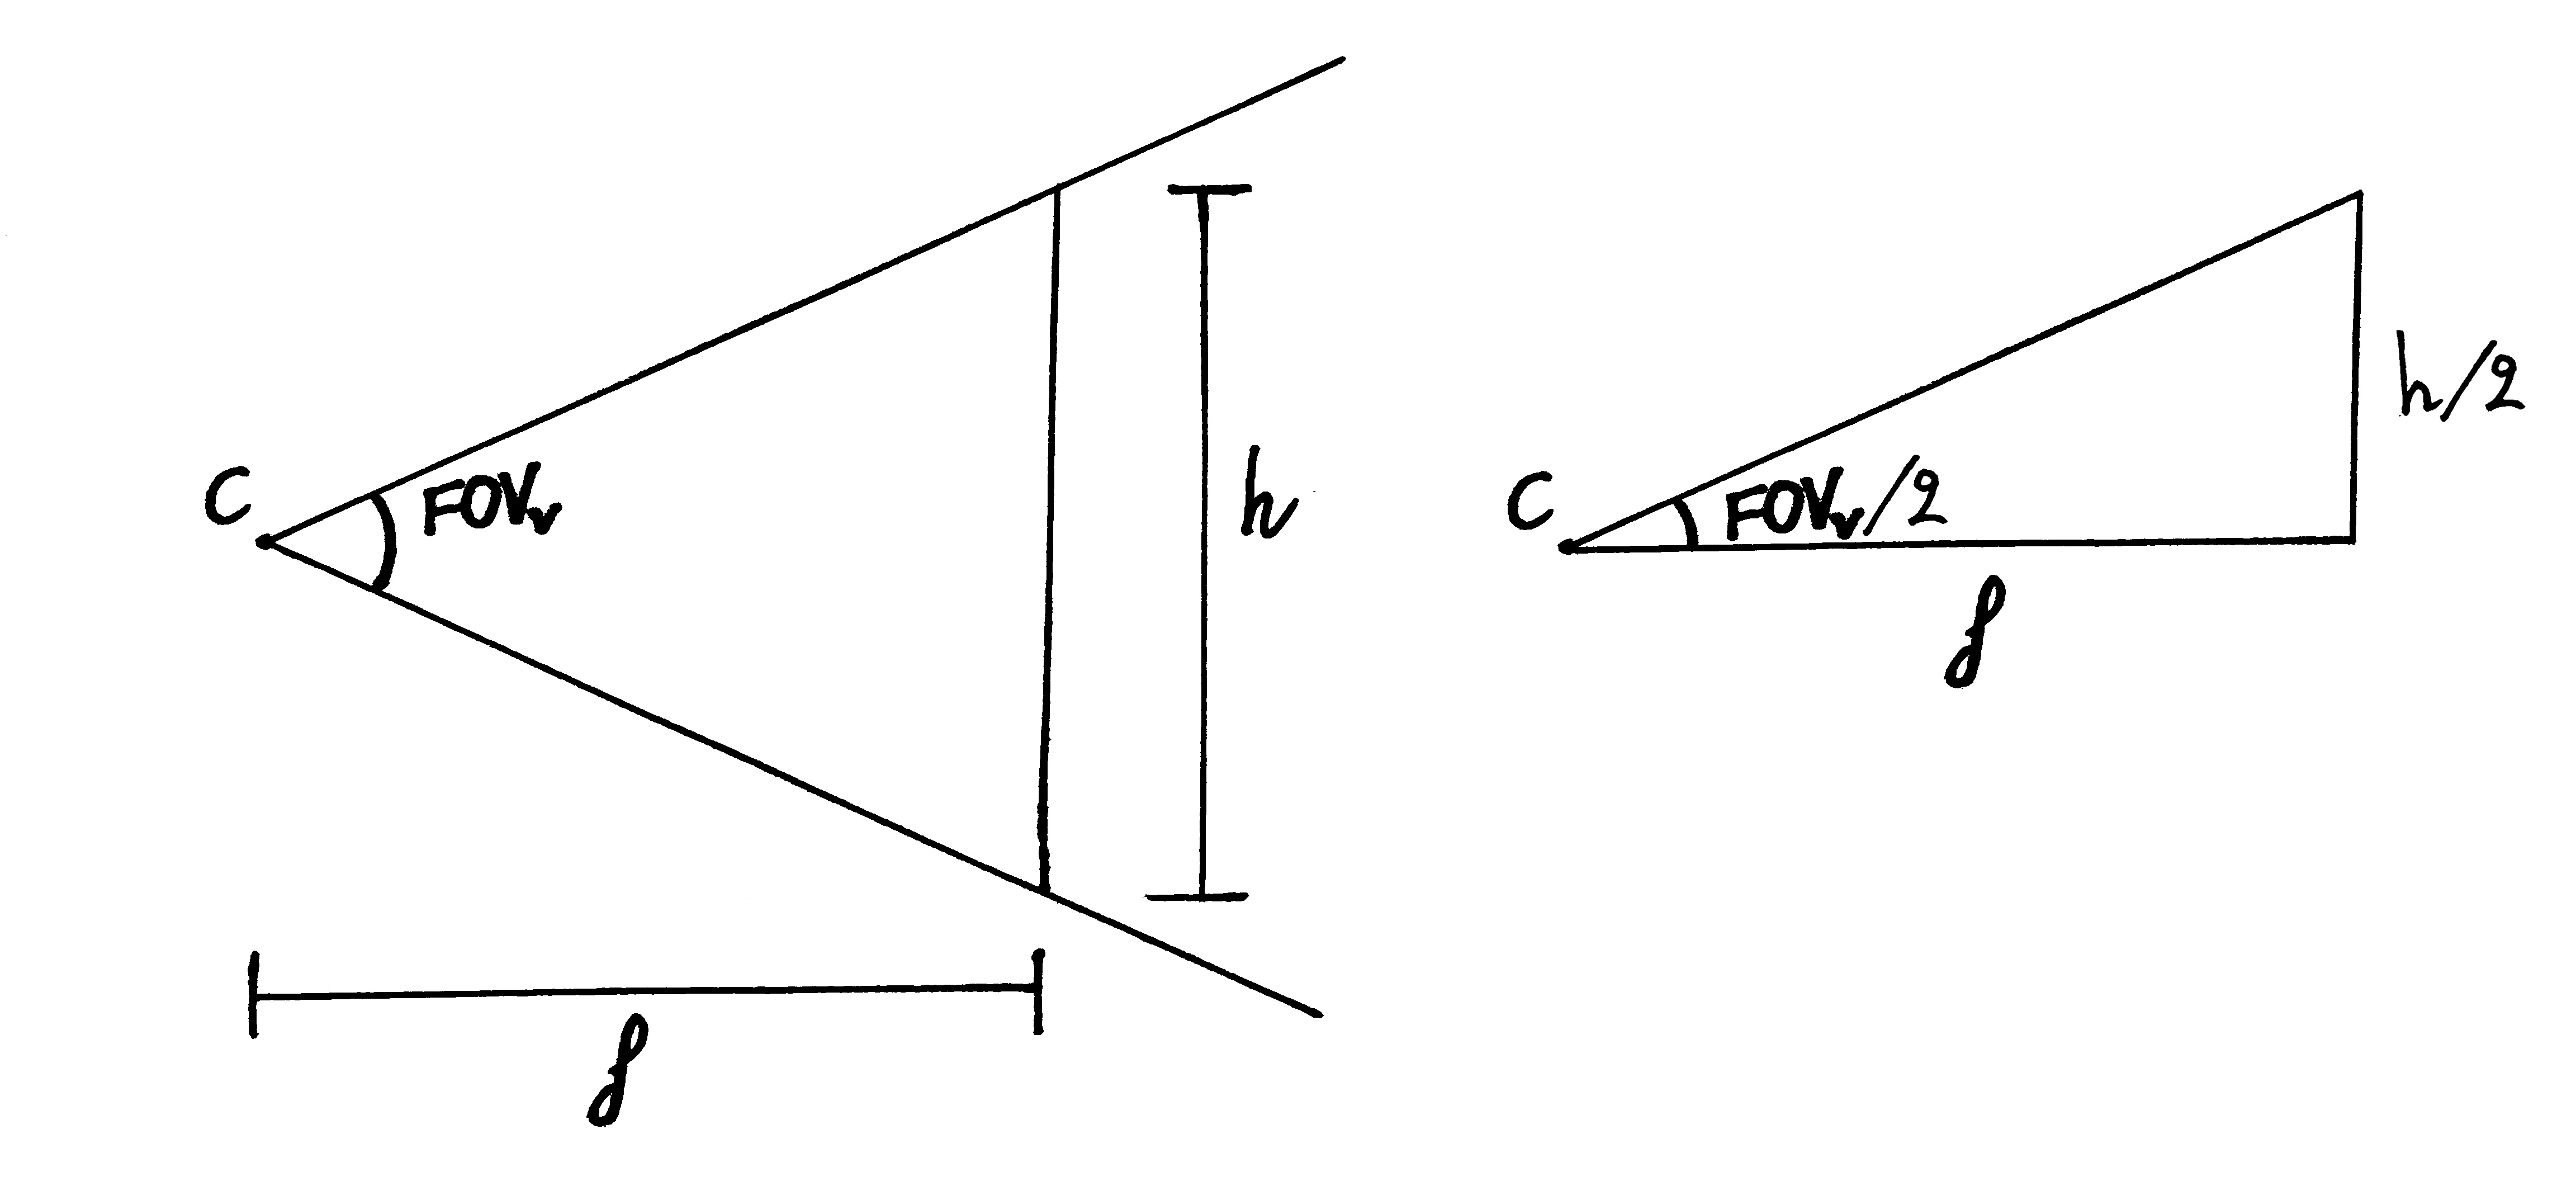
\includegraphics[width=1\textwidth]{figures/field_of_view.jpg}
    \caption{field of view (vertical)}
    \label{fig:fov}
\end{figure}
We know the dimensions of the image we capture in pixels. Solving \autoref{eq:fovv} and \autoref{eq:fovh} for $f$ we find the following equations:
\begin{equation}
    f_x = \frac{h}{2\tan(F_V/2)}
\end{equation}
\begin{equation}
    f_y = \frac{w}{2\tan(F_V/2)}
\end{equation}
Using these values, we define the following $3\times3$ matrix $\MK$ as the \textit{intrinsic parameters}:
\begin{equation}
    \MK = \begin{pmatrix}
        f_x & 0 & h_x \\
        0 & f_y & h_y \\
        0 & 0 & 1
    \end{pmatrix}
\end{equation}
These intrinsic parameters are related to a certain camera used. The projection from real world coordinates to the image coordinates (in homogeneous coordinates) can then be expressed as
\begin{equation}
    k\begin{pmatrix}
        x_{img}\\y_{img}\\1
    \end{pmatrix} = \begin{pmatrix}
        f_x & 0 & h_x & 0\\
        0 & f_y & h_y & 0\\
        0 & 0 & 1 & 0
    \end{pmatrix}\begin{pmatrix}
        X \\ Y \\ Z \\ 1
    \end{pmatrix}
\end{equation}
\begin{equation*}
    = \begin{pmatrix}
        f_x & 0 & h_x \\
        0 & f_y & h_y \\
        0 & 0 & 1
    \end{pmatrix}
    \begin{pmatrix}
        1 & 0 & 0 & 0\\
        0 & 1 & 0 & 0\\
        0 & 0 & 1 & 0\\
    \end{pmatrix}
    \begin{pmatrix}
        X \\ Y \\ Z \\ 1
    \end{pmatrix}
\end{equation*}
written more compactly:
\begin{equation}
    k\vy = \MK \biggl(\MI \lvert \vnull\biggr)\vq_c
\end{equation}

The point $\vq_c$ is expressed in the coordinate system with the principal axis of the camera pointing straight down the $X_z$-axis. At the origin of this Euclidean coordinate system, the camera is located.

\section{The general case: two views of a 3D point set}\label{sec:gen_case}
In this section I will use point-to-point correspondences between two frames. I will discuss how to get these correspondences in \autoref{chap:found_mot_est}, for now let us assume we have found these correspondences already.\bigskip

In general, we have a perspective model because we work with a camera that can be simplified to the pinhole camera model as described in \autoref{sec:cammodel}. The equations that relate motion to the image coordinates are non-linear in the motion parameters \cite{tekalp}. A two-step linear algorithm has been developed by T. S. Huang \cite{improc} in order to get the motion parameters from (at least eight) point correspondences. Doing this, an intermediate essential matrix $\ME$, consisting of the so called essential parameters is estimated. The way this algorithm works will be discussed in detail later on.

\subsubsection{Essential matrix}
The essential matrix encodes the epipolar geometry of two images. Thus, to break down the essential matrix, we need to have a look at epipolar geometry. \autoref{fig:epigeo} shows a camera in two positions $O_L$ and $O_R$. Point $X$ is projected onto the left image plane resulting in $X_L$ and onto the right image plain resulting in $X_R$.\bigskip

The points $e_L$ and $e_R$ are called the epipoles or epipolar points. They are the projection of the other camera position (its perspective center) onto the image plane. They lay on one line together with the perspective centers $O_L$ and $O_R$.\bigskip

From the perspective of $O_L$, the line $X-O_L$ is a single point $X_L$ while from the perspective of $O_R$ this is a line. This line $e_R-X_R$, shown as a red line in \autoref{fig:epigeo} is called an epipolar line.\bigskip

When the projection $X_L$ onto the left image plane is known as well as the epipolar line $e_R-X_R$ and point $X$ is projected onto the right image plane: $X_R$ evidently laying on the epipolar line, then each point observed in one image must be observed in the other image on a known epipolar line. This gives us an epipolar constraint, that for each set of points it is possible to test whether they correspond to the same 3-D point. This epipolar constraint can be described by an essential matrix.\bigskip

The essential matrix maps a point in one image to an epipolar line in the other image. If you take a point in one image and multiply it by the essential matrix, you will get the epipolar line on the other image. This essential matrix can then be decomposed into the rotation matrix and translation vector, in \autoref{ssec:essentialmat} I will discuss in detail how to estimate and then decompose the essential matrix.\bigskip

\begin{figure}
    \centering
    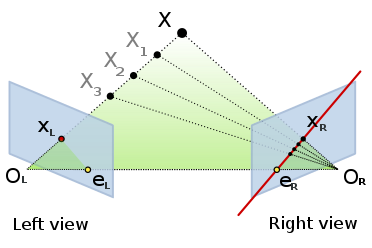
\includegraphics[width=1\textwidth]{figures/epipolar_geometry.png}
    \caption{Epipolar geometry (source: \textit{en.wikipedia.org/wiki/Epipolar\_geometry})}
    \label{fig:epigeo}
\end{figure}

Suppose we have keypoint on the image, then this keypoint corresponds with a point in the real world $\MX = (X_1, X_2, X_3)^T$ that has been matched to another keypoint corresponding to another real world point $\MX' = (X_1', X_2', X_3')^T$. The transformation of $X$ to $X'$ can be described as follows: 

\begin{equation} \label{eq:1}
    \begin{pmatrix}
        X_1' \\
        X_2' \\
        X_3'
    \end{pmatrix}
    = \MR
    \begin{pmatrix}
        X_1 \\
        X_2 \\
        X_3
    \end{pmatrix}
    + \vt
\end{equation}
where $\MR$ is the $3 \times 3$ rotation matrix and $\vt$ the translation vector.

\subsection{General case: Essential matrix}\label{ssec:essentialmat}
The OpenCV method \textit{findEssentialMat} can be used to estimate the essential matrix based on matched keypoints between two frames. In the following we will explain the way this works.\bigskip

In \cite{improc} T. S. Huang proposed that with at least eight keypoint matches a two-step linear algorithm can be developed. To do this, intermediate values called essential parameters need to be estimated first. These essential parameters form a matrix $\ME$ called the essential matrix:
\begin{equation}
    \ME = 
    \begin{pmatrix}
        e_1&e_2&e_3 \\
        e_4&e_5&e_6 \\
        e_7&e_8&e_9 
    \end{pmatrix}
    = \begin{pmatrix}
        0&-T_3&T_2 \\
        T_3&0&-T_1 \\
        -T_2&T_1&0
    \end{pmatrix}
     \MR
\end{equation}

These nine essential elements are not all independent due to the fact that  $\ME$ is a product of a skew-symmetric matrix and a rotation matrix.\bigskip

\cite{tekalp} states that vectors $\MX'$, $\vt$ and $\MR\MX$ are coplanar, since $\MX' = \MR\MX + \vt$ from (\ref{eq:1}). So now we have 
\begin{equation}
    \MX \cdot (\vt \times \MR\MX) = 0
\end{equation}
because $\vt \times \MR\MX$ is orthogonal to this plane. From this, it follows that 
\begin{equation} \label{eq:2}
    \MX'^T\ME\MX = 0
\end{equation}

We want to obtain a relationship in terms of the image plane coordinates. To do this, we divide both sides of \ref{eq:2} by $X_3 X'_3$:
\begin{equation} \label{eq:essential}
    \begin{pmatrix}
        x_1'&x_2&1
    \end{pmatrix}
    \ME
    \begin{pmatrix}
        x_1 \\
        x_2 \\
        1
    \end{pmatrix}
    = 0
\end{equation}

This linear homogeneous equation, in terms of the nine essential parameters, has either no solution or infinitely many solutions. By setting one of these nine essential parameters to one in the equation above, we can solve it for the remaining eight essential parameters. The essential parameter set to one is used as a scale factor. It is important to note that because of scale ambiguity in perspective projection, translation can only be estimated up to a scale factor.

\subsection{Estimation of the Essential Parameters}
To estimate these essential parameters, \cite{tekalp} proposes three methods: a linear lest squares method, an optimisation method requiring at least eight keypoint matches and a nonlinear method where only five, six or seven keypoint matches are needed. We'll discuss the Linear Least Squares Method.\bigskip

As stated before, one of the essential parameters will be set to one. Take $e_9 = 1$, then equation (\ref{eq:essential}) can be written as:
\begin{equation}
    \begin{pmatrix}
        x_1'x_1 &
        x_1'x_2 &
        x_1' &
        x_2'x_1 &
        x_2'x_2 &
        x_2' &
        x_1 &
        x_2
    \end{pmatrix}
    \begin{pmatrix}
        e_1 \\
        e_2 \\
        e_3 \\
        e_4 \\
        e_5 \\
        e_6 \\
        e_7 \\
        e_8 \\
    \end{pmatrix}
    = -1
\end{equation}

This linear equation in eight essential parameters can be set up as a system of $N$ linear equations in 8 unknowns. To solve this, we need at least $N \geq 8$ keypoint matches. The solution of this equation gives the essential matrix $\ME$ up to a scale factor (as discussed before). We took $e_9$ as the scale factor, but all of the other essential parameters could have been chosen as well. When using this method, $e_i, i = 1,...,9$ will be chosen based on the condition number, the $e_i$ that yields the smallest condition number will be chosen as scale factor.\bigskip

To have a solution for this equation, the coefficient matrix needs to have full rank, \cite{tekalp} states that this is the case if $\vt \neq 0$ and the shape of the 3-D surface satisfies certain conditions, called the surface constraint.

Other methods to estimate the essential parameters can be found in \cite{tekalp}.

\subsection{Decomposition of the Essential Matrix}
Now that we have the essential parameters that make up the essential matrix $\ME$, we can use this to compute rotation matrix $\MR$ and translation vector $\vt$. To do this, we rewrite $\ME$ as 

\begin{equation} \label{eq:essential2}
    \ME = 
    \begin{pmatrix}
        e1 \mid e2 \mid e3
    \end{pmatrix} = 
    \begin{pmatrix}
        k \hat{t} \times \boldsymbol{r_1} \mid
        k \hat{t} \times \boldsymbol{r_2} \mid
        k \hat{t} \times \boldsymbol{r_3} 
    \end{pmatrix}
\end{equation}

with $\boldsymbol{r_i}, i = 1, 2, 3$ are the columns of rotation matrix $\MR$, $\hat{t}$ and $k$ are the unit vector along and the length of $\vt$ respectively. \cite{tekalp} proposes a method to calculate $\MR$ and  $\hat{t}$ from noise-free as well as a method for noisy point correspondence data. As we strive to have noise-free data, we'll discuss only the first method. For the full step by step mathematical explanation, we refer to \cite{tekalp}. Here we will limit ourselves to the essential steps.\bigskip

By looking at \autoref{eq:essential2}, it is clear that each column of $\ME$ is orthogonal to $\vt$. By taking the cross product of two of the three columns, the unit vector along $\vt$ can be calculated:
\begin{equation}
    \hat{t} = \pm \frac{\boldsymbol{e_i \times e_j}}{\mid\mid e_i \times e_j\mid\mid}
    \quad i \neq j
\end{equation}

The sign of the unit vector can't be calculated with the equation above. Zhuang \cite{ZHUANG1989175} proposed the following to do so:
\begin{equation}
    \sum\begin{pmatrix}
        \hat{t} \times \begin{pmatrix}
            x_1' & x_2' & 1
        \end{pmatrix}^T
    \end{pmatrix}^T
    \cdot \ME\begin{pmatrix}
        x_1 & x_2 & 1
    \end{pmatrix}^T
    > 0
\end{equation}
the summation is taken over all observed keypoint matches.\bigskip

T. S. Huang \cite{improc} showed that 
\begin{equation}
    k^2 = \frac{1}{2}(\boldsymbol{e_1}\cdot\boldsymbol{e_1} + \boldsymbol{e_2}\cdot\boldsymbol{e_2} + \boldsymbol{e_3}\cdot\boldsymbol{e_3})
\end{equation}
Calculating $k$ this way doesn't solve the problem we had with the scale as $\boldsymbol{e_3}$ contains an arbitrary parameter but to determine the rotation parameters, we need this value for $k$.\bigskip

To calculate $\boldsymbol{r_1}$ we first calculate $\boldsymbol{e_2 \times e_3}$:
\begin{align*}
    \boldsymbol{e_2} \times \boldsymbol{e_3} = [(k\hat{t}\times \boldsymbol{r_2})\cdot\boldsymbol{r_3}]k\hat{t} - [(k \hat{t} \times \boldsymbol{r_2})k \hat{t}]\boldsymbol{r_3}
\end{align*}
The first term can be simplified as 
\begin{align}
    [(\boldsymbol{r_2}\times\boldsymbol{r_3})\cdot k\hat{t}]k\hat{t} = (\boldsymbol{r_1}\cdot k\hat{t})k\hat{t}
\end{align}
because $\boldsymbol{r_1}$, $\boldsymbol{r_2}$ and $\boldsymbol{r_3}$ are mutually orthogonal and have unity length. Since $(k\hat{t}\times\boldsymbol{r_2})$ is orthogonal to $k\hat{t}$, the second term is zero. So we have the following equations (\autoref{eq:r2} and \autoref{eq:r3} can be calculated in an analogous way):
\begin{equation}
    \boldsymbol{e_2} \times \boldsymbol{e_3} = k\hat{t}(k\hat{t}\cdot\boldsymbol{r_1})
\end{equation}
\begin{equation}\label{eq:r2}
    \boldsymbol{e_3} \times \boldsymbol{e_1} = k\hat{t}(k\hat{t}\cdot\boldsymbol{r_2})
\end{equation}
\begin{equation}\label{eq:r3}
    \boldsymbol{e_1} \times \boldsymbol{e_2} = k\hat{t}(k\hat{t}\cdot\boldsymbol{r_3})
\end{equation}

By solving these equations to $\boldsymbol{r_1}$, $\boldsymbol{r_2}$ and $\boldsymbol{r_3}$ we get the following equations:
\begin{equation}
    \boldsymbol{r_1} = \biggl[\frac{1}{k^2}\hat{t}\cdot(\boldsymbol{e_2}\times\boldsymbol{e_3})\biggr]\hat{t}+\frac{1}{k}(\boldsymbol{e_1}\times\hat{t})
\end{equation}
\begin{equation}
    \boldsymbol{r_2} = \biggl[\frac{1}{k^2}\hat{t}\cdot(\boldsymbol{e_3}\times\boldsymbol{e_1})\biggr]\hat{t}+\frac{1}{k}(\boldsymbol{e_2}\times\hat{t})
\end{equation}
\begin{equation}
    \boldsymbol{r_2} = \biggl[\frac{1}{k^2}\hat{t}\cdot(\boldsymbol{e_1}\times\boldsymbol{e_2})\biggr]\hat{t}+\frac{1}{k}(\boldsymbol{e_3}\times\hat{t})
\end{equation}\bigskip


\section{The planar case: two views of points on a plane}
Once again, as in \autoref{sec:gen_case} we will assume we have found point-to-point correspondences between two frames.\bigskip

When all points lay in one plane, the general case with the essential matrix does not work. The Essential matrix cannot be determined from such a set of points. Fortunately, there is another way to deal with this case. To do this, I need to introduce the term \newterm{homography}. \bigskip

Take a certain planar surface, when you have two images of this surface, a homography will describe the relation between that planar surface in these two images (when using the pin hole camera model). A homography is a projection between two such images.\bigskip

Such a planar surface in 3-D is defined like this:
\begin{equation}\label{eq:plane}
    n_1X_1 + n_2X_2 + n_3X_3 = 1
\end{equation}
Where $\vn = (n_1, n_2, n_3)^T$ is the normal vector of that given plane.\bigskip

A point $P = (P_1, P_2, P_3)^T$ is a point of this plane, assuming it fits in \autoref{eq:plane}. When taking an image, point $P$ will be projected onto the image plane following the pinhole camera model projection that is described by \autoref{eq:im_proj1} and \autoref{eq:im_proj2}. Accounting for the camera parameters, using \autoref{eq:improj}, each image will have its own projection of this point $P$, let us call them $P^*_1$ and $P^*_2$:
\begin{equation}
    P^*_1 = \begin{pmatrix}
        f_1 & 0 & h_{1,x} & 0\\ 
        0 & f_1 & h_{1,y} & 0\\ 
        0 & 0 & 1 & 0
    \end{pmatrix}
    \begin{pmatrix}
        P_1 \\ P_2 \\ P_3 \\ 1
    \end{pmatrix}
\end{equation}
\begin{equation}
    P^*_2 = \begin{pmatrix}
        f_2 & 0 & h_{2,x} & 0\\ 
        0 & f_2 & h_{2,y} & 0\\ 
        0 & 0 & 1 & 0
    \end{pmatrix}
    \begin{pmatrix}
        P_1 \\ P_2 \\ P_3 \\ 1
    \end{pmatrix}
\end{equation}
Note that each of these points is written in homogeneous coordinates.

The relation between these two points can be described like this:
\begin{equation}
    sP^*_1 =   \MK(\MR + \vt\vn^T)\MK^{-1}P^*_2
\end{equation}
and we define $\MH$ like this:
\begin{equation}
    \MH = (\MR + \vt\vn^T)
\end{equation}

It is possible to estimate a homography matrix if we have multiple corresponding points on both planar surfaces. It has been shown that this homography can then be decomposed into the rotation matrix, translation vector and normal vector by Huang et al. \cite{506592e3b5484e57928e215df49a83cb}. How to estimate the homography and how to decompose it will be discussed in detail in in \autoref{ssec:est_homography}.

\subsection{Planar case: Homography}\label{ssec:est_homography}

When all keypoints lie on a planar surface, we have to treat it differently as the essential matrix can not be estimated when all points lie on a single plane. When all points lie on a planar surface, we can use that fact that a homography $\MH$ describes the transformation of that planar surface. For this we only look at the points below the horizon on the road surface. Then all keypoints lie on a plane that can be described as
\begin{equation}
    aX_1 + bX_2 + cX_3 = 1
\end{equation}
where $(a, b, c)^T$ is the normal vector of this plane. \autoref{eq:1} can then be rewritten as 
\begin{equation}
    \begin{pmatrix}
        X_1' \\
        X_2' \\
        X_3'
    \end{pmatrix} = \MR
    \begin{pmatrix}
        X_1 \\
        X_2 \\
        X_3
    \end{pmatrix} + \vt
    \begin{pmatrix}
        a & b & c
    \end{pmatrix}
    \begin{pmatrix}
        X_1 \\
        X_2 \\
        X_3
    \end{pmatrix}
\end{equation}
or
\begin{equation}
    \begin{pmatrix}
        X_1' \\
        X_2' \\
        X_3'
    \end{pmatrix} =
    \begin{pmatrix}
        a_1 & a_2 & a_3 \\
        a_4 & a_5 & a_6 \\
        a_7 & a_8 & a_9 \\
    \end{pmatrix}
    \begin{pmatrix}
        X_1 \\
        X_2 \\
        X_3
    \end{pmatrix} = \MA
    \begin{pmatrix}
        X_1 \\
        X_2 \\
        X_3
    \end{pmatrix}
\end{equation}
with
\begin{equation} \label{eq:matrixA}
    \MA = \MR + \vt
    \begin{pmatrix}
        a & b & c
    \end{pmatrix}
\end{equation}

$a_1,...,a_9$ are called the pure parameters \cite{506592e3b5484e57928e215df49a83cb}. As with the computation of the essential parameters, the scale ambiguity problem is also present here so we normalise $a_9 = 1$. The 3-D displacement is projected onto a 2-D plane using the perspective transformation. The mapping of 3-D displacement $t$ to 2-D image plane $t'$ is given by 
\begin{equation*}
    x_1' = \frac{a_1x_1 + a_2x_2 + a_3}{a_7x_1 + a_8x_2 + 1}
\end{equation*}
\begin{equation}\label{eq:pure}
     x_2' = \frac{a_4x_1 + a_5x_2 + a_6}{a_7x_1 + a_8x_2 + 1}
\end{equation}

\subsection{Estimation of the pure parameters}
\autoref{eq:pure} can be rearranged by cross-multiplying the equations for each keypoint match:
\begin{equation}
    \begin{pmatrix}
        x_1 & x_2 & 1 & 0 & 0 & 0 & -x_1x_1' & -x_2x_1' \\
        0 & 0 & 0 & x_1 & x_2 & 1 & -x_1x_2' & -x_2x_2'
    \end{pmatrix}
    \begin{pmatrix}
        a_1 \\ a_2 \\ a_3 \\ a_4 \\ a_5 \\ a_6 \\ a_7 \\ a_8 \\
    \end{pmatrix} = 
    \begin{pmatrix}
        x_1' \\ x_2'
    \end{pmatrix}
\end{equation}
So if we have at least four keypoint matches, eight or more linear equations can be set up to solve for the pure parameters. \cite{improc} showed that the rank of the matrix is 8 if and only if no three of the four observed points are collinear in three dimensions.

\subsection{Estimation of the motion and structure parameters}
We now have found the pure parameters and thus matrix $\MA$. As \autoref{eq:matrixA} states, motion parameters $\MR$ and $\vt$ can be derived from $\MA$, as well as the normal vector $(a,b,c)^T$. To do this, we need to decompose $\MA$ using singular value decomposition (SVD). \cite{Huang:86} describes describes a method to do this:

First of all, we write matrix $\MA$ as 
\begin{equation}
    \MA = \MU
    \begin{pmatrix}
        \lambda_1 & 0 & 0 \\
        0 & \lambda_2 & 0 \\
        0 & 0 & \lambda_3
    \end{pmatrix}\MV^T
\end{equation}

where $\MU = (\boldsymbol{u_1}\mid\boldsymbol{u_2}\mid\boldsymbol{u_3})$ and $\MV = (\boldsymbol{v_1}\mid\boldsymbol{v_2}\mid\boldsymbol{v_3})$ are $3\times 3$ orthogonal matrices and $\lambda_1\geq\lambda_2\geq\lambda_3\geq 0$ are the singular values of $\MA$. Depending on the multiplicity of the singular values there are 3 different cases.

\subsubsection{Multiplicity of singular values is 1: $\lambda_1 > \lambda_2 > \lambda_3$}

This indicates that the motion can be decomposed into a rotation around an axis through the origin and a translation in a direction, not along the normal vector. In this case, there are two possible solutions for the pure parameters:
\begin{equation*}
    \MR = \MU
    \begin{pmatrix}
        \alpha & 0 & \beta \\
        0 & 1 & 0 \\
        -s\beta & 0 & s\alpha
    \end{pmatrix}
    \MV^T
\end{equation*}
\begin{equation*}
    \vt = k\biggl(-\beta\boldsymbol{u_1} + (\frac{\lambda_3}{\lambda_2}-s\alpha)\boldsymbol{u_3}\biggr)
\end{equation*}
\begin{equation*}
    \begin{pmatrix}
        a & b & c
    \end{pmatrix}^T = \frac{1}{k}(\delta\boldsymbol{v_1} + \boldsymbol{v_3})
\end{equation*}
with
\begin{equation*}
    \alpha = \frac{\lambda_1 + s\lambda_3\delta^2}{\lambda_2(1+\delta^2)}
\end{equation*}
\begin{equation*}
    \beta = \frac{1}{\delta}\biggl(\alpha-\frac{\lambda_1}{\lambda_2}\biggr)
\end{equation*}
\begin{equation*}
    \delta = \pm\biggl(\frac{\lambda_1^2-\lambda_2^2}{\lambda_2^2-\lambda_3^2}\biggr)^\frac{1}{2}
\end{equation*}
\begin{equation*}
    s = \det{\MU} \det{\MV}
\end{equation*}
and $k$ is an arbitrary scale factor (either positive or negative). To resolve the scale ambiguity, $1/X_3 > 0$ is required for all points.

\subsubsection{Multiplicity of singular values is 2: $\lambda_1 = \lambda_2 \neq \lambda_3$}
This indicates that the motion can be decomposed into a rotation around an axis through the origin and a translation along the normal vector. Now a unique solution for the motion parameters exist:
\begin{equation*}
    \MR = \frac{1}{\lambda_1}\MA-\biggl(\frac{\lambda_3}{\lambda_1}-s\biggr)\boldsymbol{u_3}\boldsymbol{v_3^T}
\end{equation*}
\begin{equation*}
    \vt = k\biggl(\frac{\lambda_3}{\lambda_1}-s\biggr)
\end{equation*}
\begin{equation*}
    \begin{pmatrix}
        a & b & c
    \end{pmatrix}^T = \frac{1}{k}\boldsymbol{v_3}
\end{equation*}
\begin{equation*}
    s = \det{\MU} \det{\MV}
\end{equation*}
Once again, $k$ is an arbitrary scale factor.
\subsubsection{Multiplicity of singular values is 2: $\lambda_1 = \lambda_2 = \lambda_3$}
This indicates the rotation is a pure rotation around an axis through the origin. Once again, there's a unique solution for the rotation matrix:
\begin{equation*}
    \MR = \left(\frac{1}{\lambda_1}\right)\MA
\end{equation*}
In this case, it is not possible to determine translation vector $\vt$ and the normal vector $(a, b, c)^T$ as there is no translation.

\section{Combining the use of homography and essential matrix}
Using one of these does not have to exclude using the other. As the footage we will be using will have both points laying on a fixed planar surface (being the road surface) and points spread out in space, we can use the essential matrix and homography matrix complementary.
